

\section{System Architecture}

\begin{figure}[ht!]
\centering
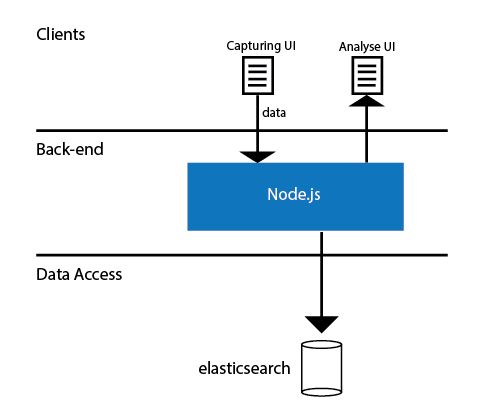
\includegraphics[width=100mm]{images/general/arhitecture.png}
\caption{}
\label{overflow}
\end{figure}

\subsection{Domain model}



\subsection{Storage}

The data storage is an elasticsearch database. Elasticsearch is document oriented and works extremely well with JSON. As our server is built on JavaScript working with JSON is easy. JSON-objects can be inserted right into the storage and elasticsearch will map fields and value accordingly.  Our data input is generated in the web browser which also uses JavaScript and could have been inserted right away into the database without any pre mapping.
Elasticsearch takes advantages of embedded documents meaning we can store related data together. As an attack is usually made up of several passes you can store the passes as an embedded document inside the attack document so they can be retrieved in one query. 

The main reason for using Elasticsearch is its search capability. In a single query you can get counted how many passes all player for a team has played and received, number of times all players has been the breakthrough-player, type of attacks, most used zones for passing and finishing and so on. This makes it very easy and efficient to do queries for analyses on teams and players. After a query you can return all data directly to the client for him to expose to the end user.

\subsection{Back-end}

The back end is the middleware between the clients and the data layer. It exposes a RESTful interface over HTTP for the client to communicate. A request coming in is transformed to a database query based on the resource it tries to access. On answer from the database the result is transformed before returning it to the client. 

Similar if the client sends new data for a match the middle-ware inserts the data into the appropriate indexes.


\subsection{Front-end}

Front end is consist of a single page JavaScript application using Backbone.js as under-supporting framework. As it uses a MVC structure the models is responsible for AJAX communication with the back-end. 

For a analytic toolkit to be sufficient a good UI is critical. Here several helper library is used to present the data. HighCharts.js is JavaScript library for illustrating graphs. A query on team generates a lot of statistics and rather than listing them up they are presented using charts. 

BILDE AV CHART
\begin{figure}[ht!]
\centering
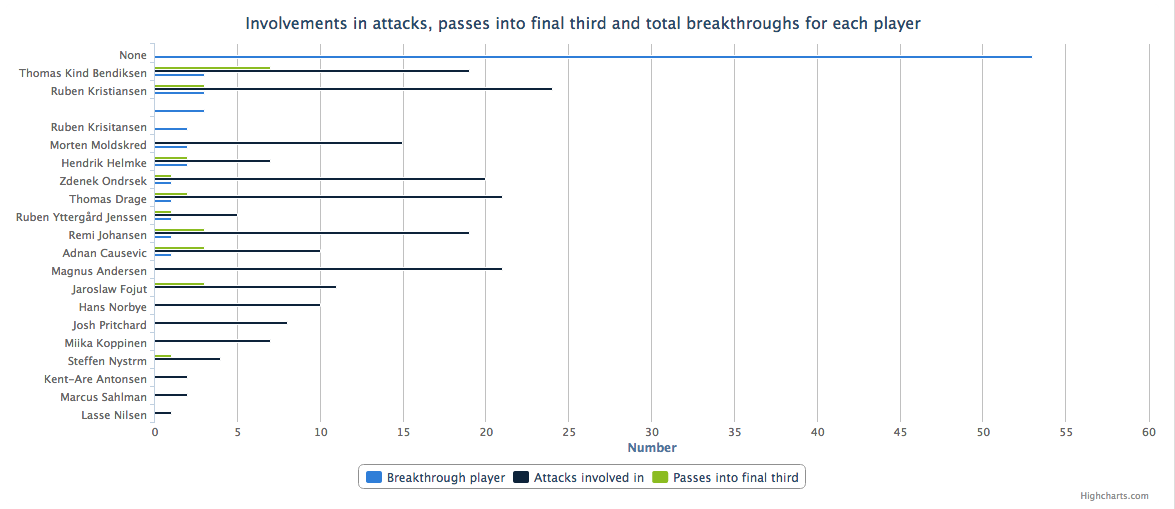
\includegraphics[width=100mm]{images/general/chart_passes.png}
\caption{Shows how the pass statistic is illustrated on the client by using HighCharts.js}
\label{overflow}
\end{figure}


Positional data is created using the new feature of HTML5, canvas. 


\subsubsection{Domain Model}


\subsubsection{Elasticsearch}


\subsubsection{Security}
Secturity is not handled. This means anyone getting into the page can post new match data. 